\documentclass[superscriptaddress,floatfix,onecolumn,notitlepage]{revtex4-1}
\usepackage{epsfig,hyperref,graphics,float,amsmath,mathtools}
\usepackage{setspace,siunitx,physics,epsfig,graphicx}
\usepackage[caption=false]{subfig}
\usepackage{color}
\usepackage{nameref}
\usepackage[cm]{fullpage}
\usepackage[section]{placeins}
\captionsetup[subfigure]{labelformat=brace}
\renewcommand{\thefigure}{S\arabic{figure}}
\begin{document}
\bibliographystyle{apsrev4-1}

\title{\textit{Supplemental Materials:} A Chiral, Incommensurate Helical Phase
in a Smectic of Achiral Bent-Core Mesogens}
\date{\today}
\author{Adam~A.~S.~Green}
\affiliation{Department of Physics and Soft Materials Research Center,
University of Colorado Boulder, Boulder, CO, 80309-0390, USA}
\author{Michael~R.~Tuchband}
\affiliation{Department of Physics and Soft Materials Research Center,
University of Colorado Boulder, Boulder, CO, 80309-0390, USA}
\author{Renfan~Shao}
\affiliation{Department of Physics and Soft Materials Research Center,
University of Colorado Boulder, Boulder, CO, 80309-0390, USA}
\author{Yongqiang~Shen}
\affiliation{Department of Physics and Soft Materials Research Center,
University of Colorado Boulder, Boulder, CO, 80309-0390, USA}
\author{Rayshan~Visvanathan}
\affiliation{Department of Physics and Soft Materials Research Center,
University of Colorado Boulder, Boulder, CO, 80309-0390, USA}
\author{Alexandra~E. Duncan}
\affiliation{Department of Physics and Soft Materials Research Center,
University of Colorado Boulder, Boulder, CO, 80309-0390, USA}
\author{Anne~Lehmann}
\affiliation{Department of Chemistry, Martin Luther University
Halle-Wittenberg, D-06120 Halle, Germany}
\author{Carsten~Tschierske}
\affiliation{Department of Chemistry, Martin Luther University
Halle-Wittenberg, D-06120 Halle, Germany}

\author{Eric~D.~Carlson}
\affiliation{Department of Chemistry and Soft Materials Research Center,
University of Colorado Boulder, Boulder, CO, 80309-0215, USA}

\author{Edward~Guzman}
\affiliation{Department of Chemistry and Soft Materials Research Center,
University of Colorado Boulder, Boulder, CO, 80309-0215, USA}

\author{Maria~Kolber}
\affiliation{Department of Chemistry and Soft Materials Research Center,
University of Colorado Boulder, Boulder, CO, 80309-0215, USA}

\author{David~M.~Walba}
\affiliation{Department of Chemistry and Soft Materials Research Center,
University of Colorado Boulder, Boulder, CO, 80309-0215, USA}

\author{Cheol~S.~Park}
\affiliation{Department of Physics and Soft Materials Research Center,
University of Colorado Boulder, Boulder, CO, 80309-0390, USA}
\author{Matthew~A.~Glaser}
\affiliation{Department of Physics and Soft Materials Research Center,
University of Colorado Boulder, Boulder, CO, 80309-0390, USA}

\author{Joseph~E.~Maclennan}
\affiliation{Department of Physics and Soft Materials Research Center,
University of Colorado Boulder, Boulder, CO, 80309-0390, USA}

\author{Noel~A.~Clark}
\affiliation{Department of Physics and Soft Materials Research Center,
University of Colorado Boulder, Boulder, CO, 80309-0390, USA}


\newcommand{\smapr}[1]{$\mathrm{SmAP}_\mathrm{R}$}
\newcommand{\sma}[1]{$\mathrm{SmA}$}
%\newcommand{\smc}[1]{$\mathrm{SmC}$}
\newcommand{\smapf}[1]{$\mathrm{SmAP}_\mathrm{F}$}
\newcommand{\smapa}[1]{$\mathrm{SmAP}_\mathrm{A}$}
\newcommand{\smcapalp}[1]{$\mathrm{SmC}_\textrm{A}\textrm{P}_\mathrm{\alpha}$}
\newcommand{\smapalp}[1]{$\mathrm{SmAP}_\mathrm{\alpha}$}
\newcommand{\smcapf}[1]{$\mathrm{SmC}_\textrm{A}\textrm{P}_\mathrm{F}$}
\newcommand{\smcspf}[1]{$\mathrm{SmC}_\textrm{S}\textrm{P}_\mathrm{F}$}
\newcommand{\smcspa}[1]{$\mathrm{SmC}_\textrm{S}\textrm{P}_\mathrm{A}$}
\newcommand{\smchph}[1]{$\mathrm{Sm(CP)}_\alpha$}

\newcommand{\smcrpr}[1]{$\text{de Vries SmA}$}

\newcommand{\smchphM}[1]{\mathrm{Sm(CP)}_\alpha}
\newcommand{\smcdpd}[1]{$\mathrm{SmC}_\textrm{D}\textrm{P}_\mathrm{D}$}
\newcommand{\smcdpdM}[1]{\mathrm{SmC}_\textrm{D}\textrm{P}_\mathrm{D}}
\newcommand{\smcapa}[1]{$\mathrm{SmC}_\textrm{A}\textrm{P}_\mathrm{A}$}
\newcommand{\smcapaprime}[1]{$\mathrm{SmC}_\textrm{A}\textrm{P}_\mathrm{A'}$}
\newcommand{\smaprM}[1]{\mathrm{SmAP}_\mathrm{R}}
\newcommand{\smaM}[1]{\mathrm{SmA}}
\newcommand{\smapfM}[1]{\mathrm{SmAP}_\mathrm{F}}
\newcommand{\smapaM}[1]{\mathrm{SmAP}_\mathrm{A}}
\newcommand{\smapalpM}[1]{\mathrm{SmAP}_\mathrm{\alpha}}
\newcommand{\smcapfM}[1]{\mathrm{SmC}_\textrm{A}\textrm{P}_\mathrm{F}}
\newcommand{\smcspfM}[1]{\mathrm{SmC}_\textrm{S}\textrm{P}_\mathrm{F}}
\newcommand{\smcspaM}[1]{\mathrm{SmC}_\textrm{S}\textrm{P}_\mathrm{A}}
\newcommand{\smcapaM}[1]{\mathrm{SmC}_\textrm{A}\textrm{P}_\mathrm{A}}

\newcommand{\smcapaprimeM}[1]{\mathrm{SmC}_\textrm{A}\textrm{P}_\mathrm{A`}}

\newcommand{\nsix}[1]{\textbf{n-16}}
\newcommand{\nfour}[1]{\textbf{PAL30}}
\newcommand{\smcp}[2]{SmC$_\text{#1}$P$_\text{#2}$}
\newcommand{\smap}[1]{SmAP$_\text{#1}$}


\maketitle
%
\section{Experimental Methods}
We used a combination of two-dimensional, small-angle, hard X-ray scattering
(SAXS),  resonant, soft X-ray scattering (RSoXS), polarized, transmitted light microscopy on cells in transmission, and measurements of the polarization reversal current of cells in order to characterize \nfour{phi}.


The RSoXS experiments were performed at the Advanced Light Source at Lawrence
Berkeley National Laboratory beamline 11.0.1.2 using linearly polarized X-ray
photons~\cite{wang2011defining, liu2016resonant}. The X-ray energy was tuned
between \SI{270}{\eV} and \SI{290}{\electronvolt} in our experiments, with
scattering contrast appearing only for energies near the carbon K-edge resonance (E =
\SI{284}{\electronvolt}), indicating the presence of real-space features with an orientational modulation.
The \nfour{phi} material was sandwiched between two silicon nitride substrates,
while in the isotropic phase. The cell was then placed into a temperature
controlled hotstage in the beamline.
After finding the highest temperature where scattering features were observed,
the sample was cooled slowly while recording $2$D diffractograms of the scattering. The
RSoXS setup is sensitive to orientational modulations from $d=$ \SIrange{50}{1250}{\angstrom}. The relative positions and orientations of the sample and detector were calibrated using a
sample with known scattering $q$-values. The data from the detector was processed using the
Igor Pro-based NIKA data reduction software package~ \cite{ilavsky2012nika, zhang2010glassy}.

The angular resolution of the diffractometer, estimated from the full width at
half-maximum of a resonant feature known to be twice the smectic layer spacing
is $\delta q \sim \SI{.00078}{\angstrom^{-1}}$.

SAXS measurements were carried out on beamline X10A of the National Synchrotron
Light Source (NSLS), at Brookhaven National Laboratory. This beamline has a Si 111 double monochromator, tuned to around \SI{10}{\kilo\electronvolt}. The sample was mounted in an Instec hot stage on a Huber four-circle goniometer.
%
The angular resolution of the diffractometer, measured by scanning the detector arm
through the attenuated direct beam, is $\delta q \sim
\SI{0.005}{\nano\metre^{-1}}$ full width at half-maximum.

The planar cells used for texture analysis were \SI{4.5}{\micro\metre} thick commercial cells purchased from Instec Inc.\ with rubbed polyimide planar alignment layers and ITO glass. The thickness of the empty cells was measured using a visible light spectrometer. The cells were then filled with \nfour{phi} in the isotropic phase.  Polarization reversal current was measured in these cells by applying an alternating, triangular voltage.

The birefringence was measured using a Zeiss quartz-wedge compensator and a
\SI{5.86}{\micro\metre} thick Instec cell.

The molecular length of \nfour{phi} was estimated using a Hartree-Fock 6-31G*
calculation of a single molecule in the gas phase using the Spartan ‘16
numerical calculation package.

\clearpage

\section{Supplemental Figures}

\begin{figure}[H]
    \centering
    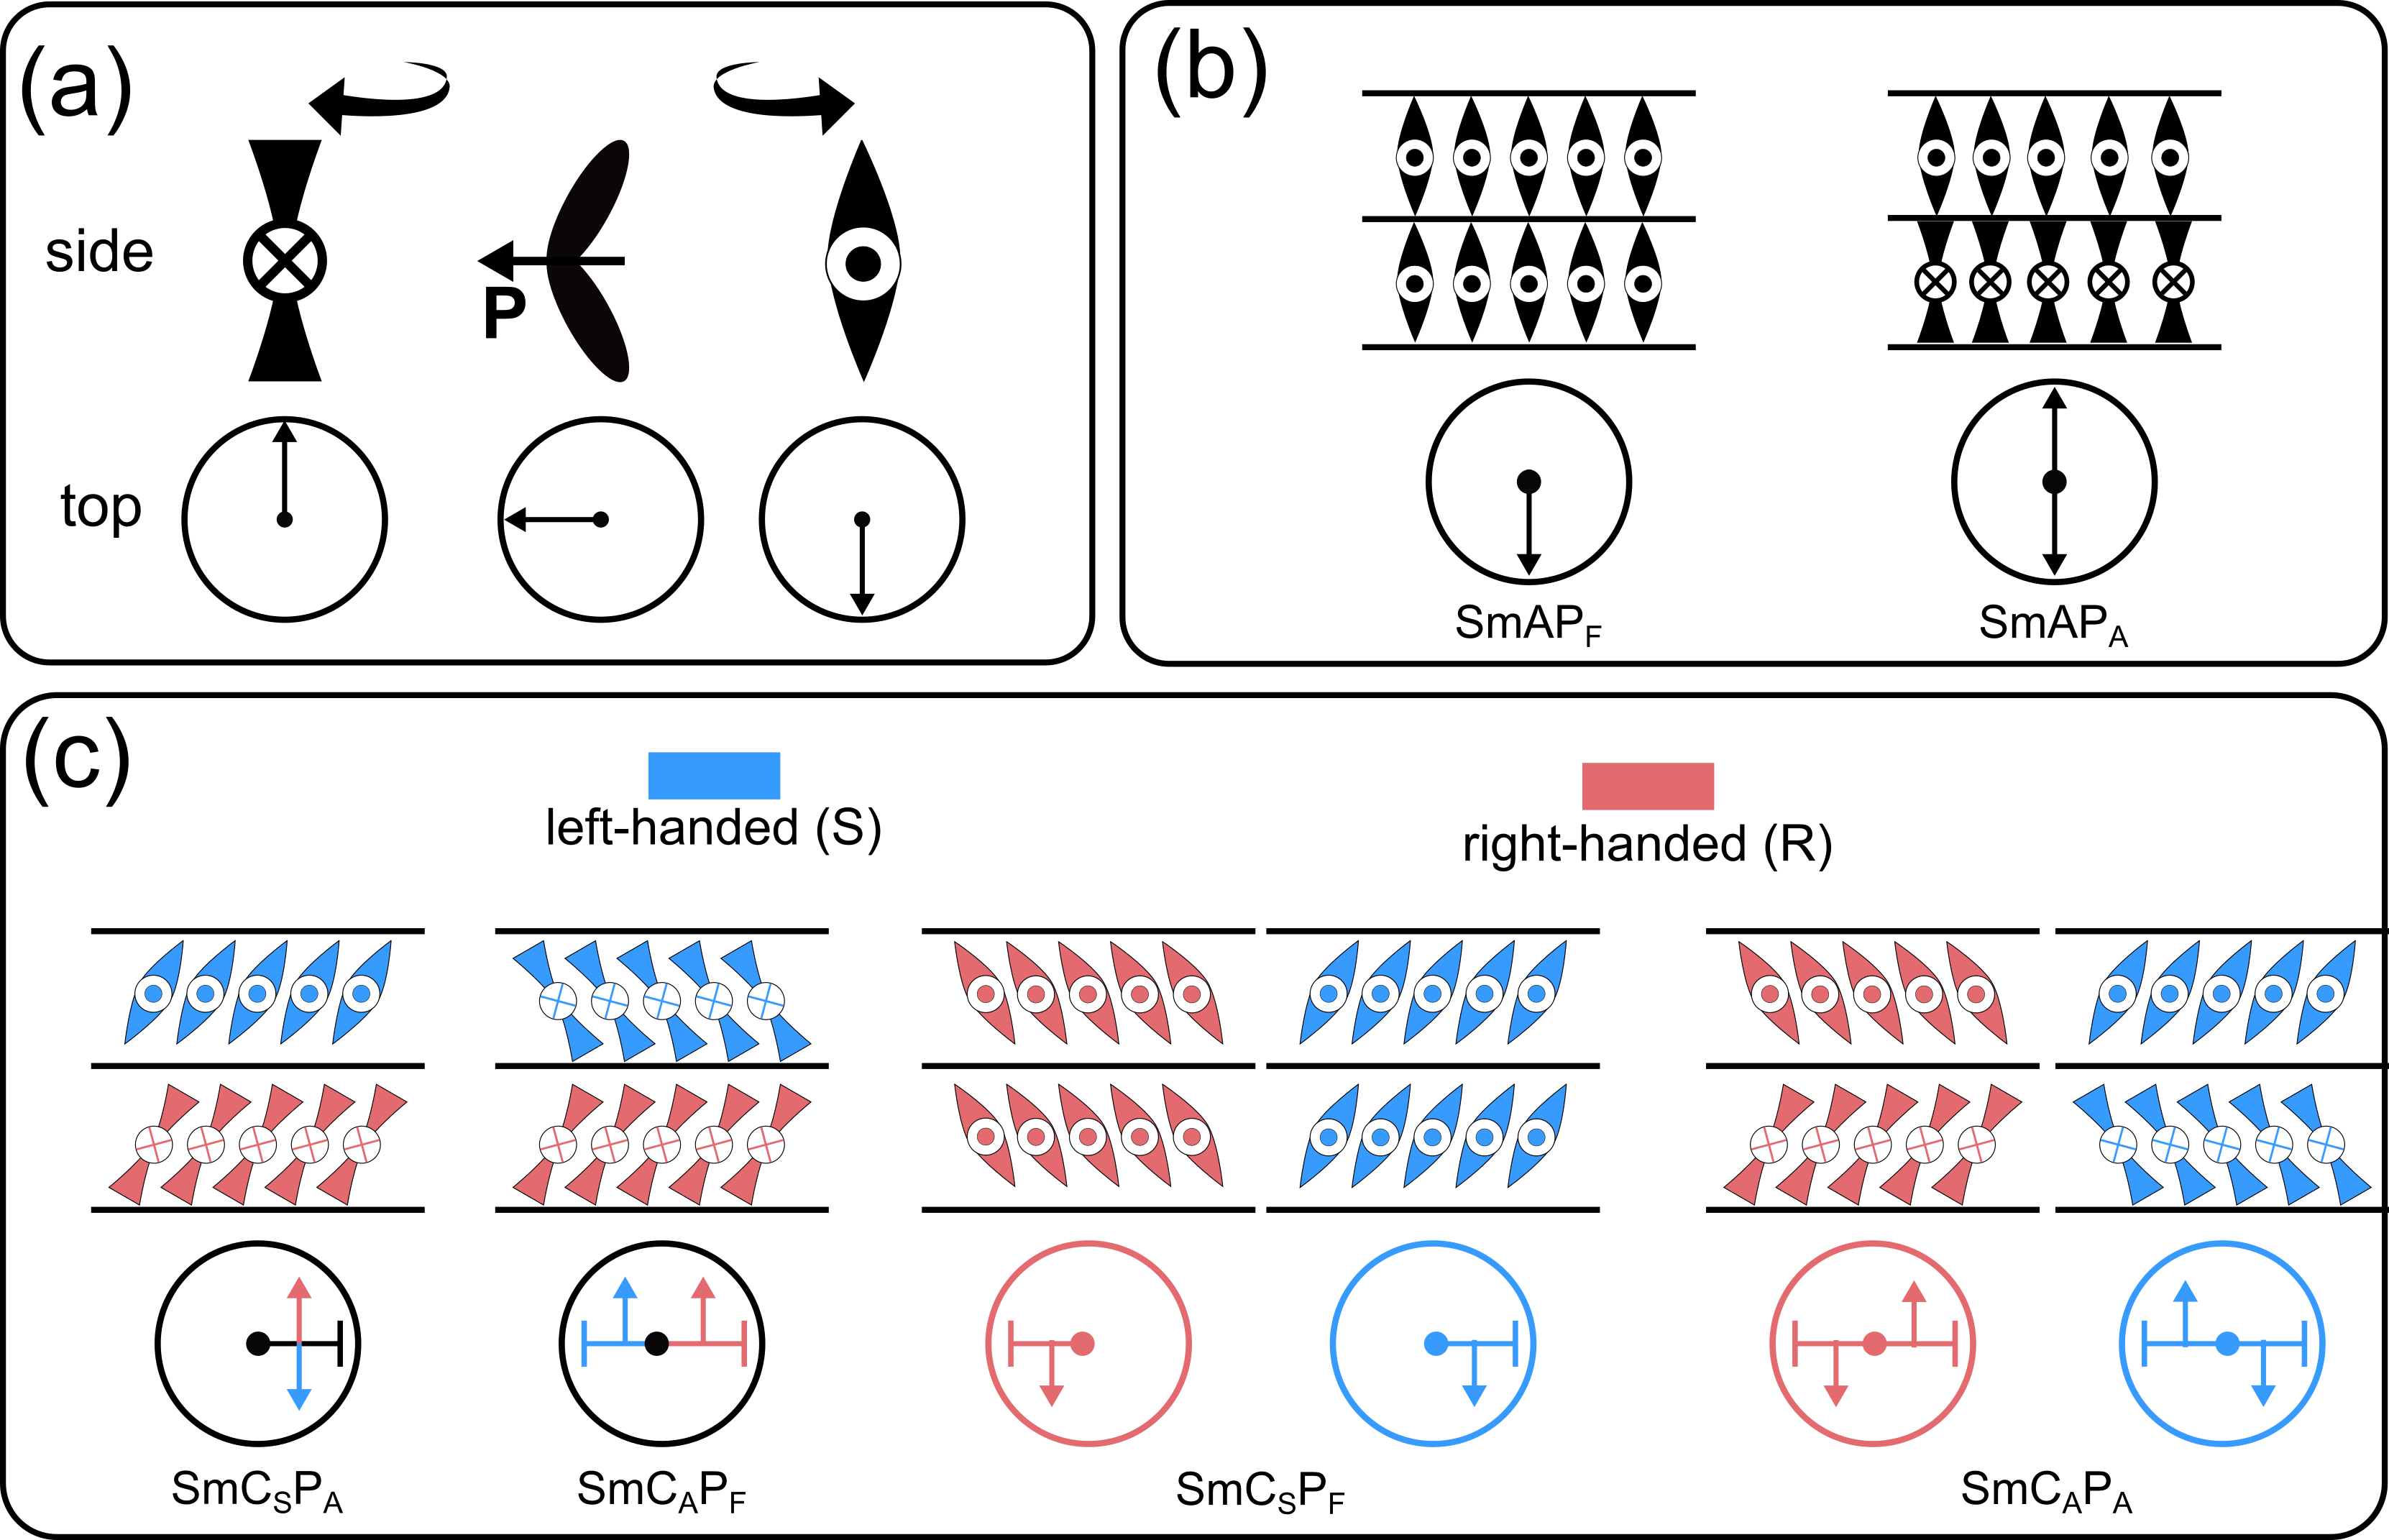
\includegraphics[width=.7\textwidth]{bent-core-phase-diagrams-suppFinal.png}
    \caption{Tilt and polarity of selected bent-core smectic phases. (a) Generic
    bent-core molecule at various orientations. (b) Polar orthogonal  phases.
    (c) Tilted states of the B2 phase.
    The tilt director is indicated by $\dashv$  and the polar vector by $\rightarrow$.
    The smectic layers are colored according to their chirality, with black being achiral or
    racemic, blue left-handed, and red
     right-handed. }
\end{figure}

\begin{figure}[H]
    \centering
    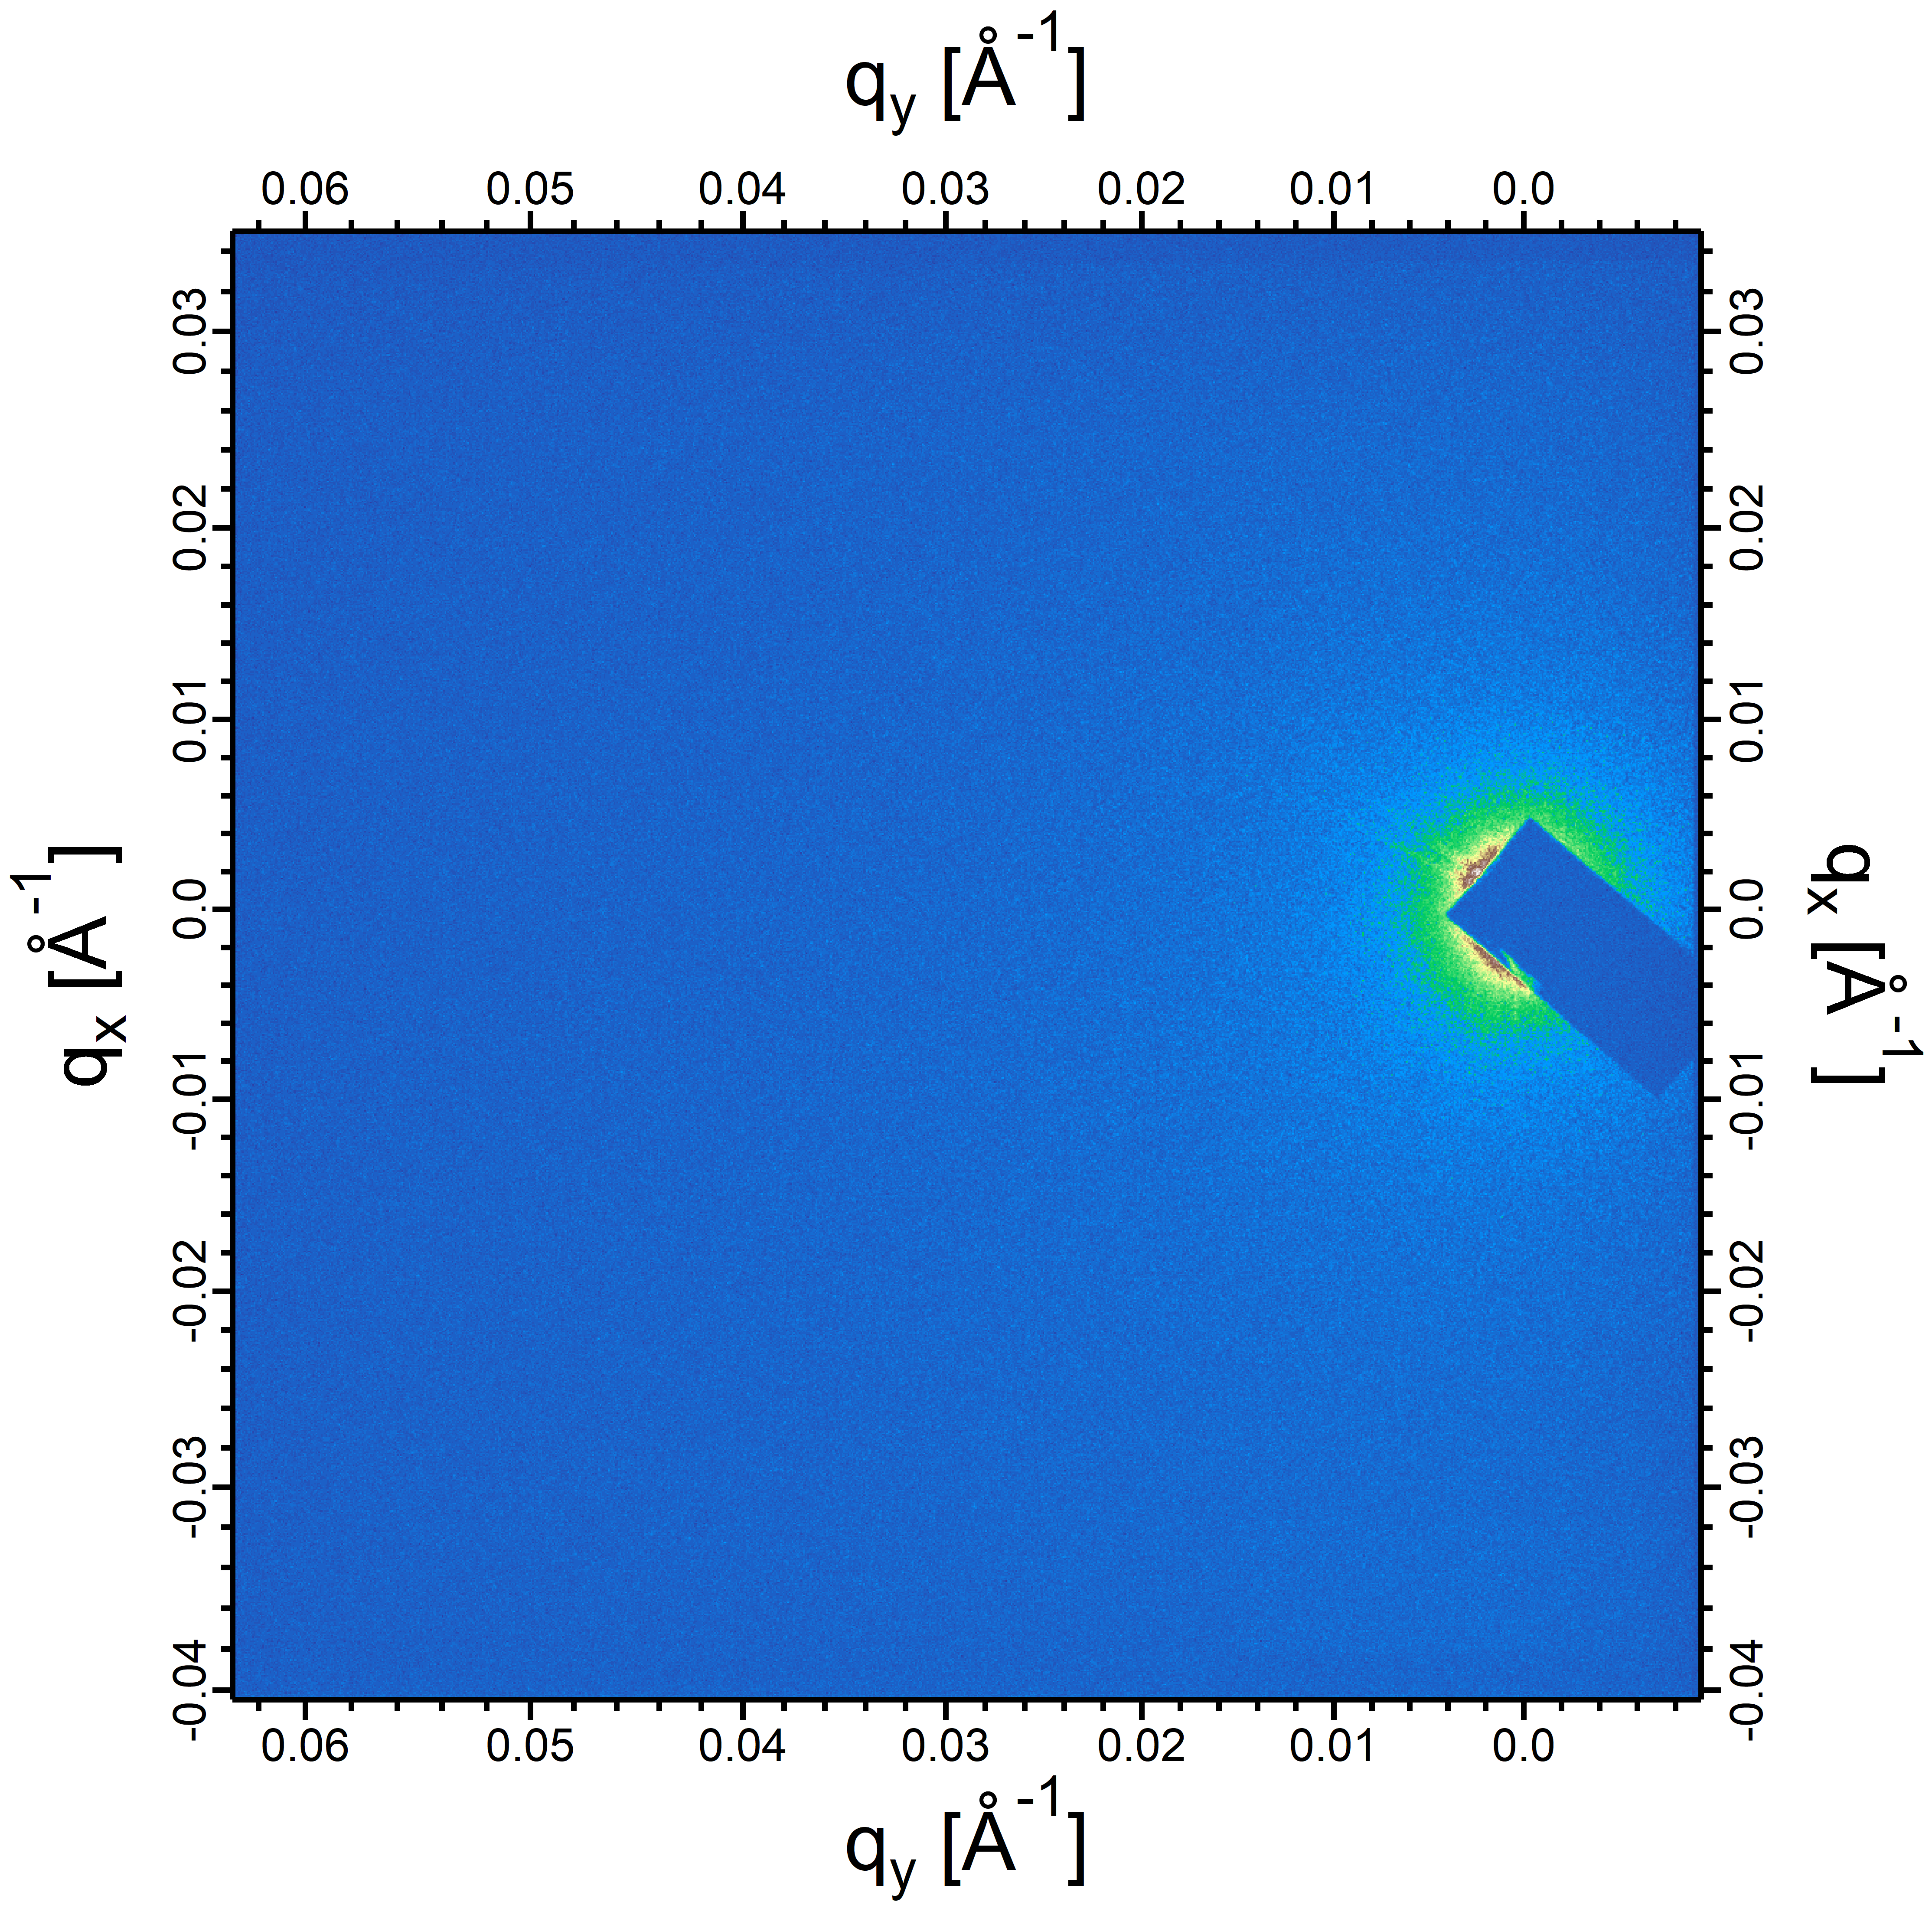
\includegraphics[width=.5\textwidth]{rsosxSmaT113-modified.png}
    \caption{Resonant soft X-ray scattering (RSoXS) of \nfour{phi} observed in
        the Sm1 phase ($T=\SI{113}{\degreeCelsius}$). This image is
        characteristic of the phase. The absence of any
        resonant scattering features is characteristic of the Sm1 showing that
        there are no periodic
    structures present.}
\end{figure}


\begin{figure}[H]
    \centering
    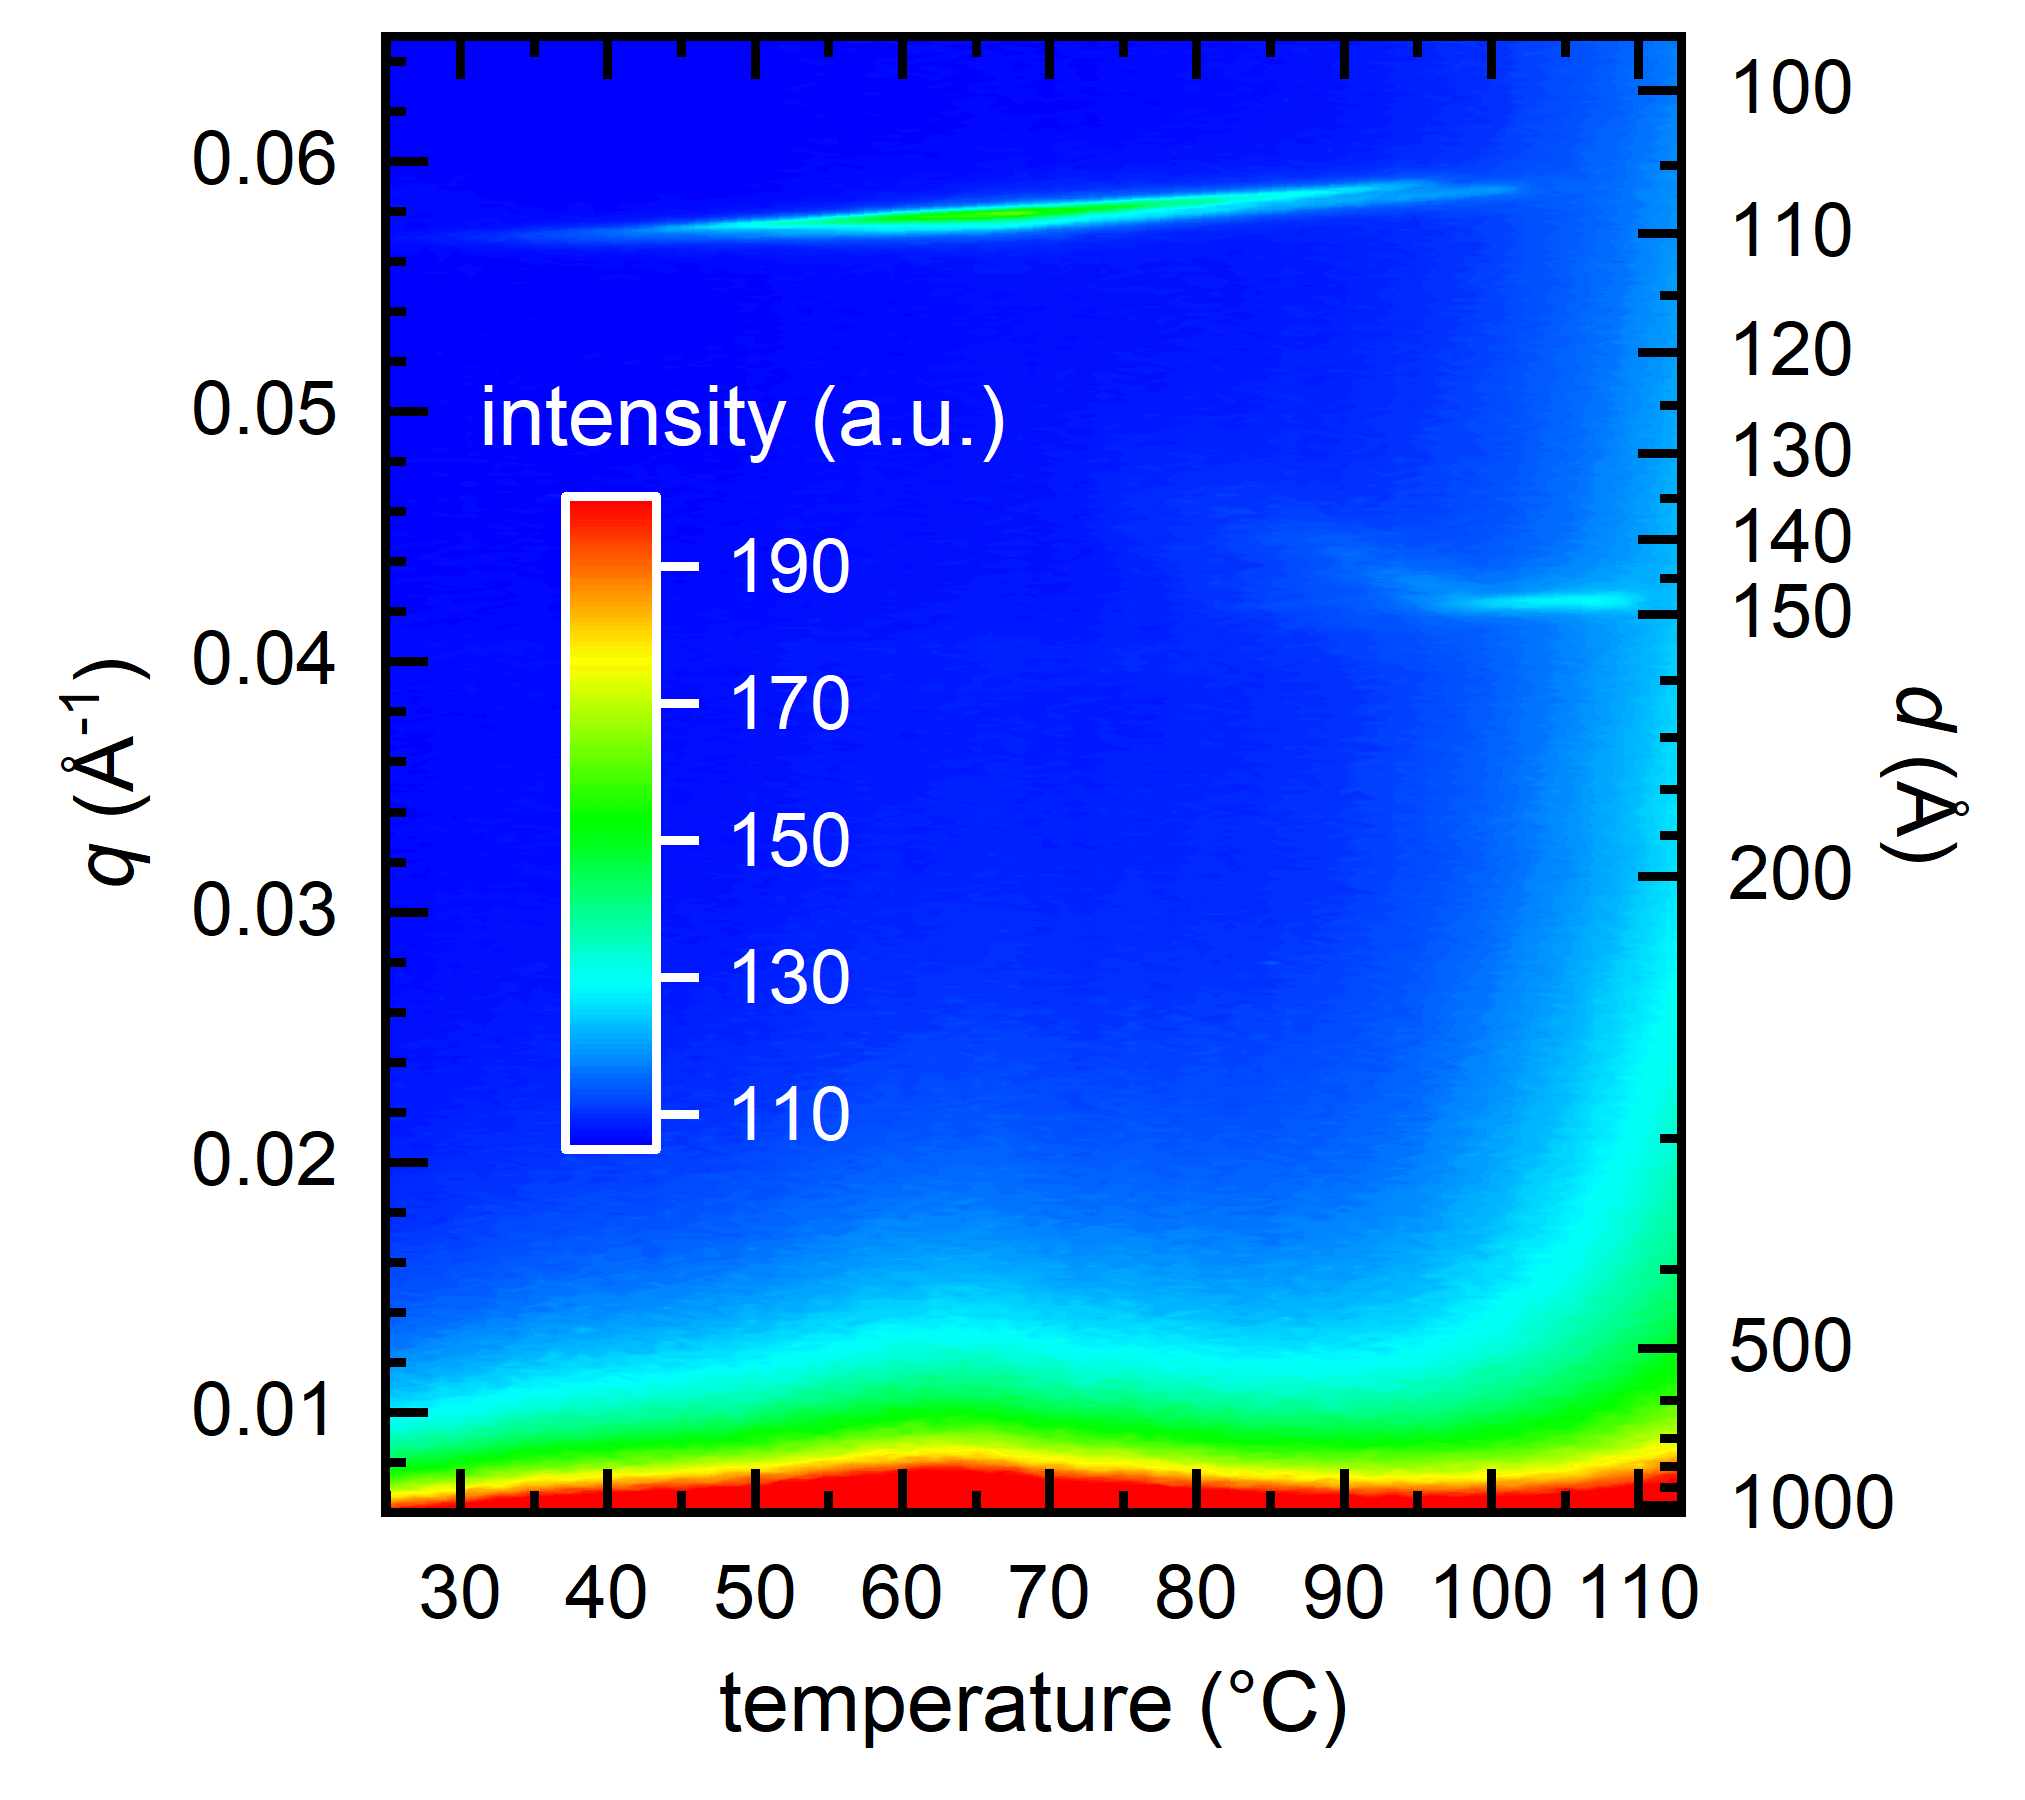
\includegraphics[width=.5\textwidth]{PAL30RSOXSshiftedTcontourplotv1mt.png}
    \caption{Resonant soft X-ray scattering (RSoXS) of \nfour{phi} observed
        vs.\ temperature on
    cooling. The plot was generated
    from a temperature series of 2D diffractograms that were azimuthally
    averaged, then interpolated and plotted in $q$-space with corresponding real-space coordinates
    ($d=2\pi/q$). Above \SI{110}{\degreeCelsius}, we
    observe no scattering features, indicating the absence of resonant structures periodic in
    this $d$-range. On cooling below \SI{110}{\degreeCelsius}, a scattering arc
    appears at $d=\SI{148}{\angstrom}$, corresponding to  about three smectic layer
    spacings.
    This reflection persists on further cooling but becomes weaker and
    disappears
    at \SI{99}{\degreeCelsius}. At
    \SI{105}{\degreeCelsius}, a second feature appears (at $d =
    \SI{107}{\angstrom}$)
    corresponding to two smectic layer spacings. This feature
    shifts to smaller $q$, and then disappears at the transition to the
    crystal phase at \SI{65}{\degreeCelsius}. In the $q$ range we investigated
    (corresponding to \SIrange{50}{1256}{\angstrom}), we see no other orientational modulations.}
\end{figure}

\begin{figure}[H]
    \centering
    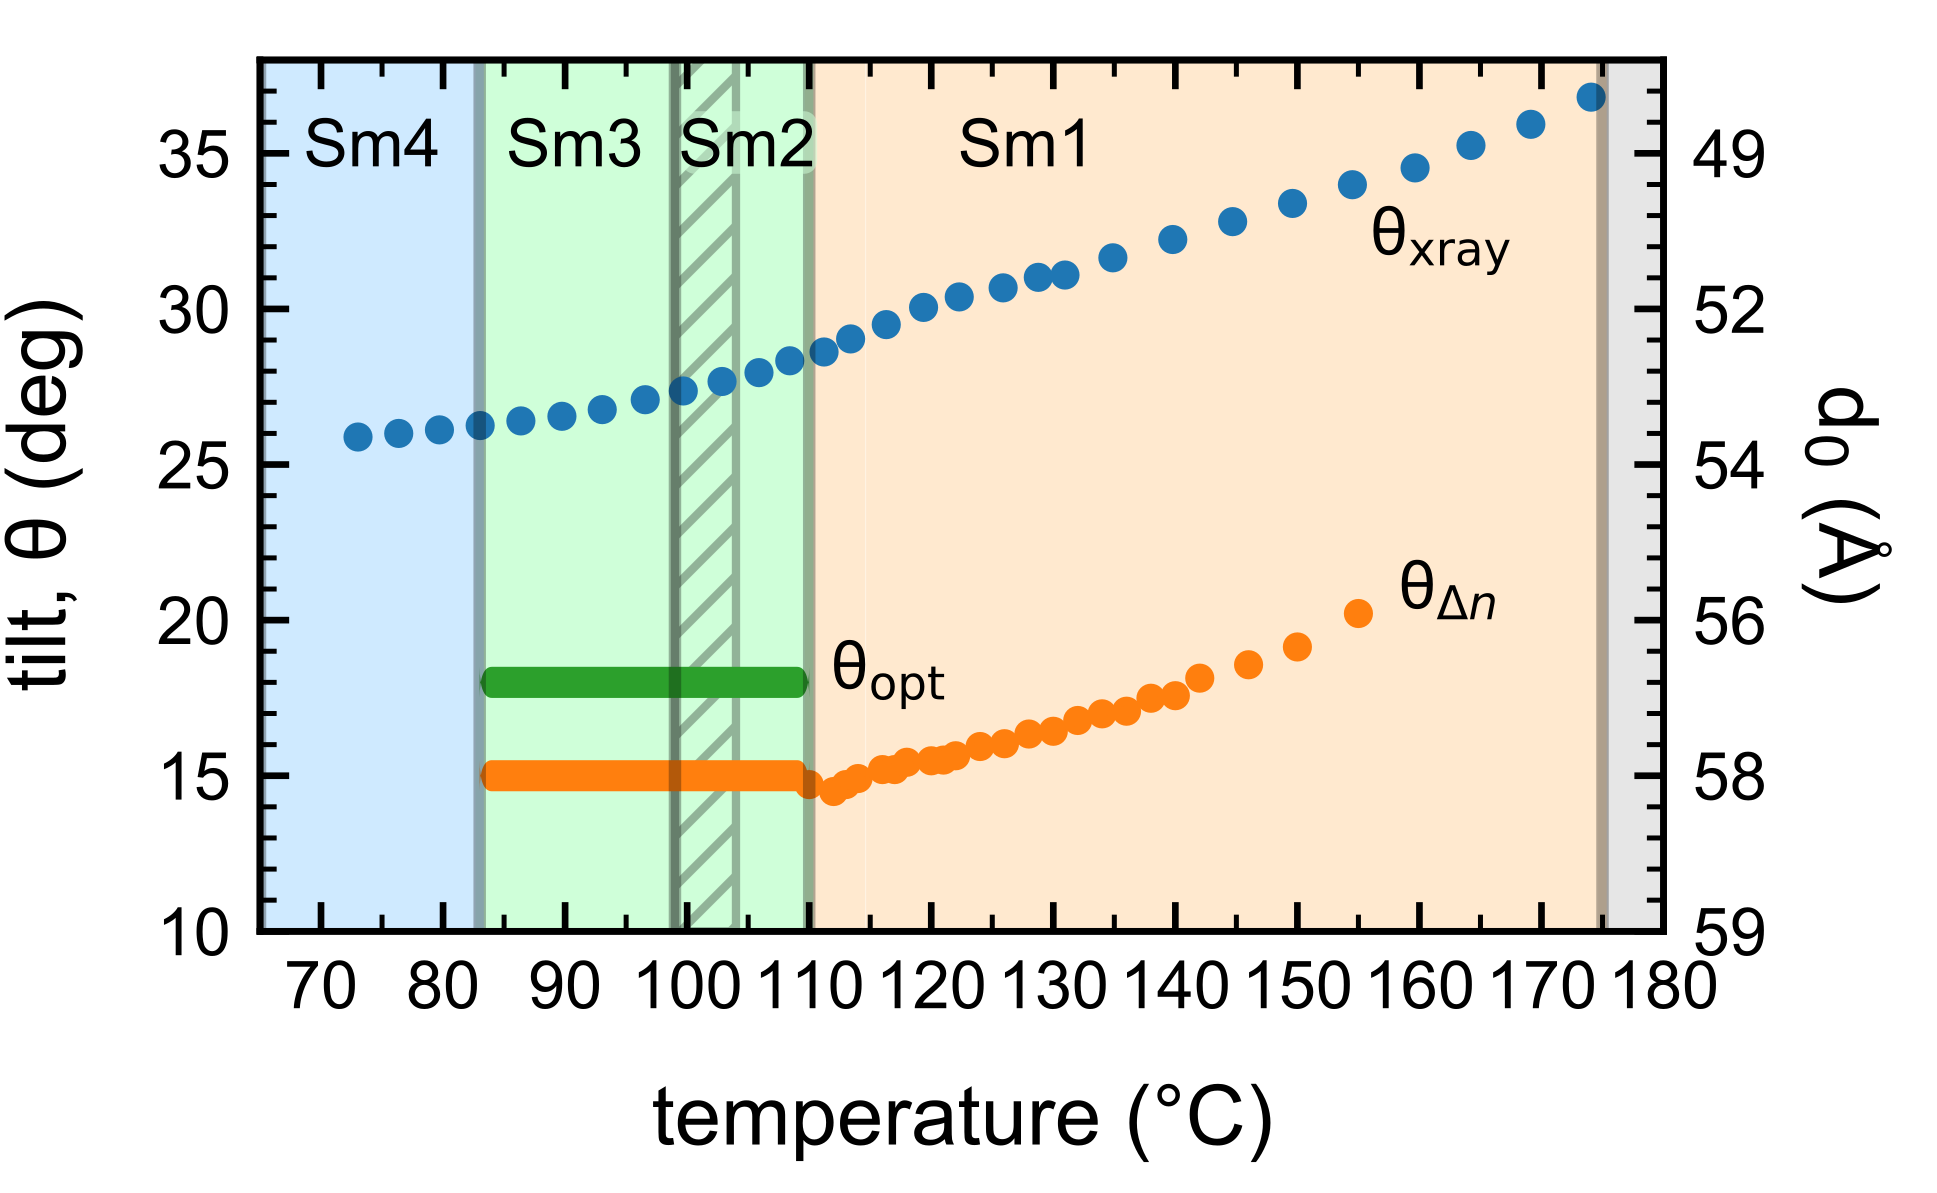
\includegraphics[width=.7\textwidth]{tilt-master.png}

    \caption{Molecular tilt of \nfour{phi} as a function of temperature. The
        X-ray tilt is found using, $\theta_\text{xray} =
        \arccos(d_0/l_\text{calc})$, where $d_0$ is the smectic
        layer spacing measured by SAXS and $l_\text{calc} =
        \SI{59.9}{\angstrom}$ is the fully-trans calculated
    length from Spartan. The layer
    spacing (X-ray tilt) increases (decreases) monotonically on cooling.
Even the highest value for the
    layer spacing ($d_0\approx \SI{54}{\angstrom}$), is still significantly less than the
    predicted molecular length $l_\text{calc}=\SI{59.9}{\angstrom}$, suggesting
    that there may be a significant
    degree of intercalation or tilt present in all smectic phases. The fact that
    the Sm2 is chiral
    suggests that Sm2 \textit{must} be tilted. Because the dramatic
    changes of the layer spacing that would be expected at a transition between
    an orthogonal and a tilted phase are not seen anywhere in the SAXS
    temperature scan, every smectic phase should also show comparable tilt.
The fact that the measured optical tilt ($\theta_\text{opt}$) is less than
    the tilt calculated from the layer spacing, $\theta_\text{xray}$ suggests a significant degree of
    intercalation is also present.}
\end{figure}


\begin{figure}[H]
    \centering
    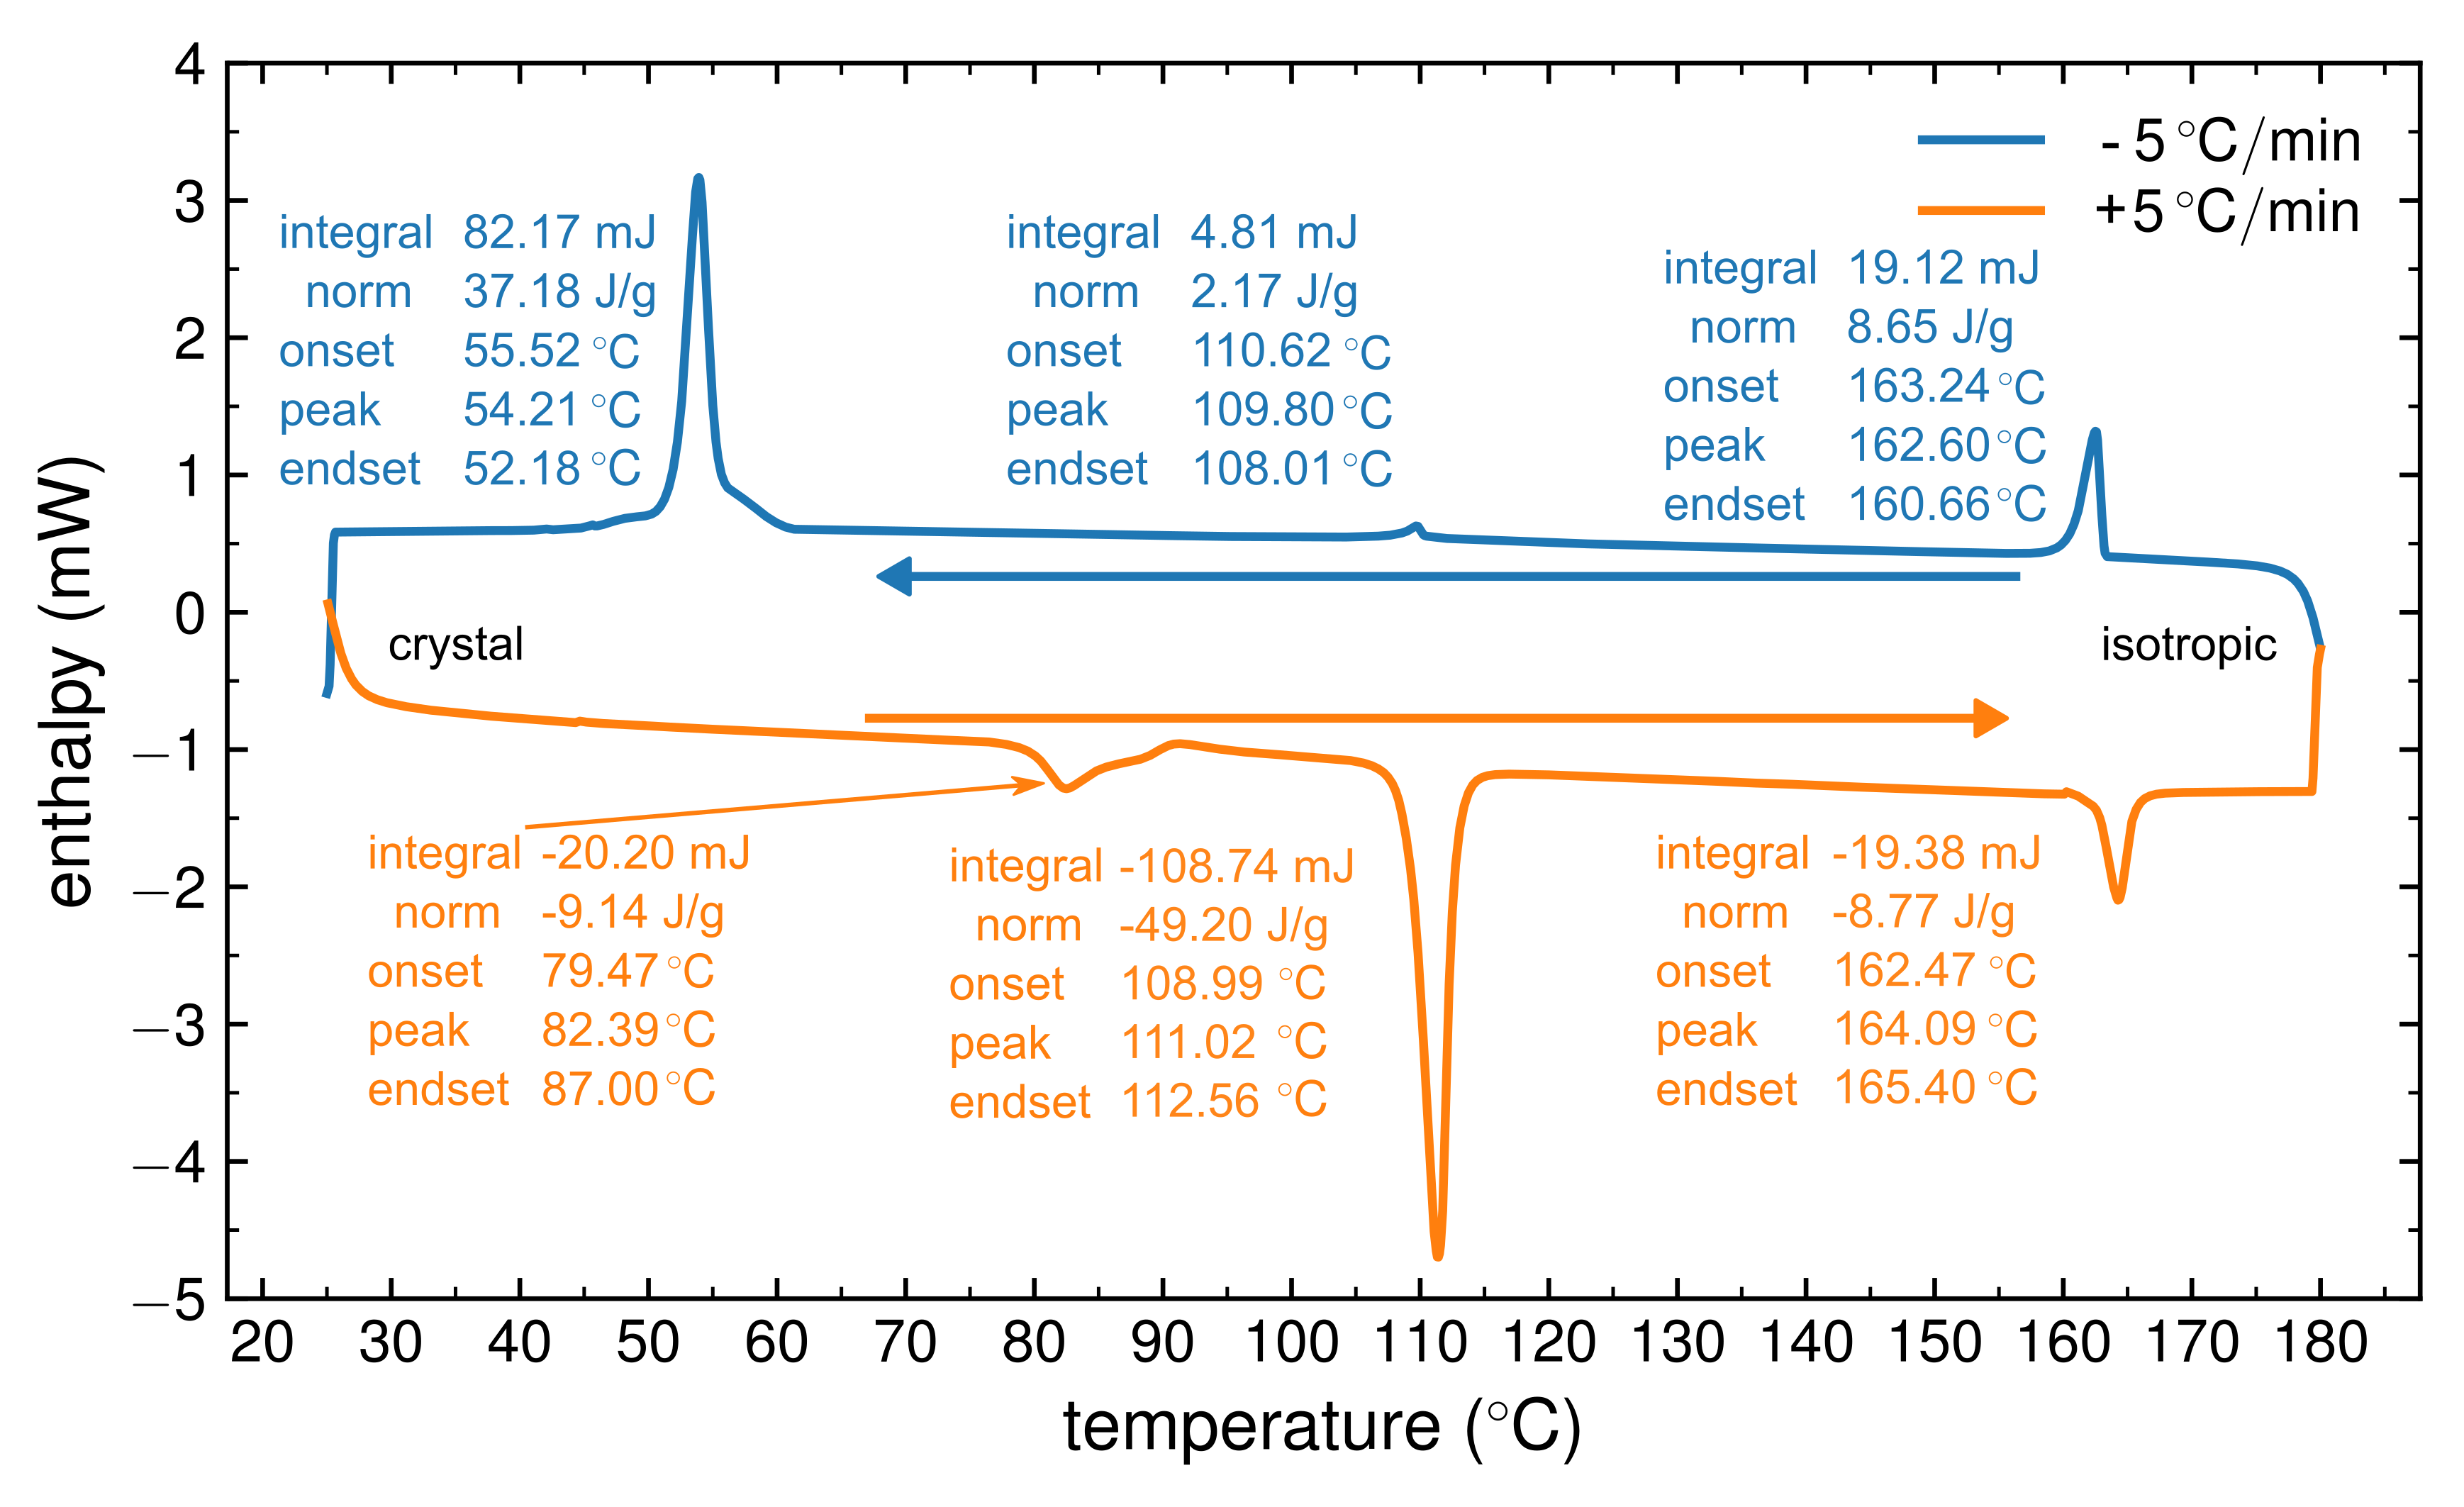
\includegraphics[width=.7\textwidth]{dsc-slowrunFinal.png}
    \caption{Differential scanning calorimetry (DSC) of \nfour{} on slow cooling
    and heating.
    Since \nfour{} appears to be monotropic, all
    experimental characterization described in this paper was carried out on cooling, between the clearing point
    (\SI{162}{\degreeCelsius}) and crystallization
    (\SI{54.21}{\degreeCelsius}).
    The peak observed on cooling at \SI{109.8}{\degreeCelsius}
    corresponds to the transition from the \smcrpr{phi} to the
    \smchph{phi} phase.
    The enthalpy of the other transitions was too small to be detected.}
\end{figure}

\begin{figure}[H]
    \centering
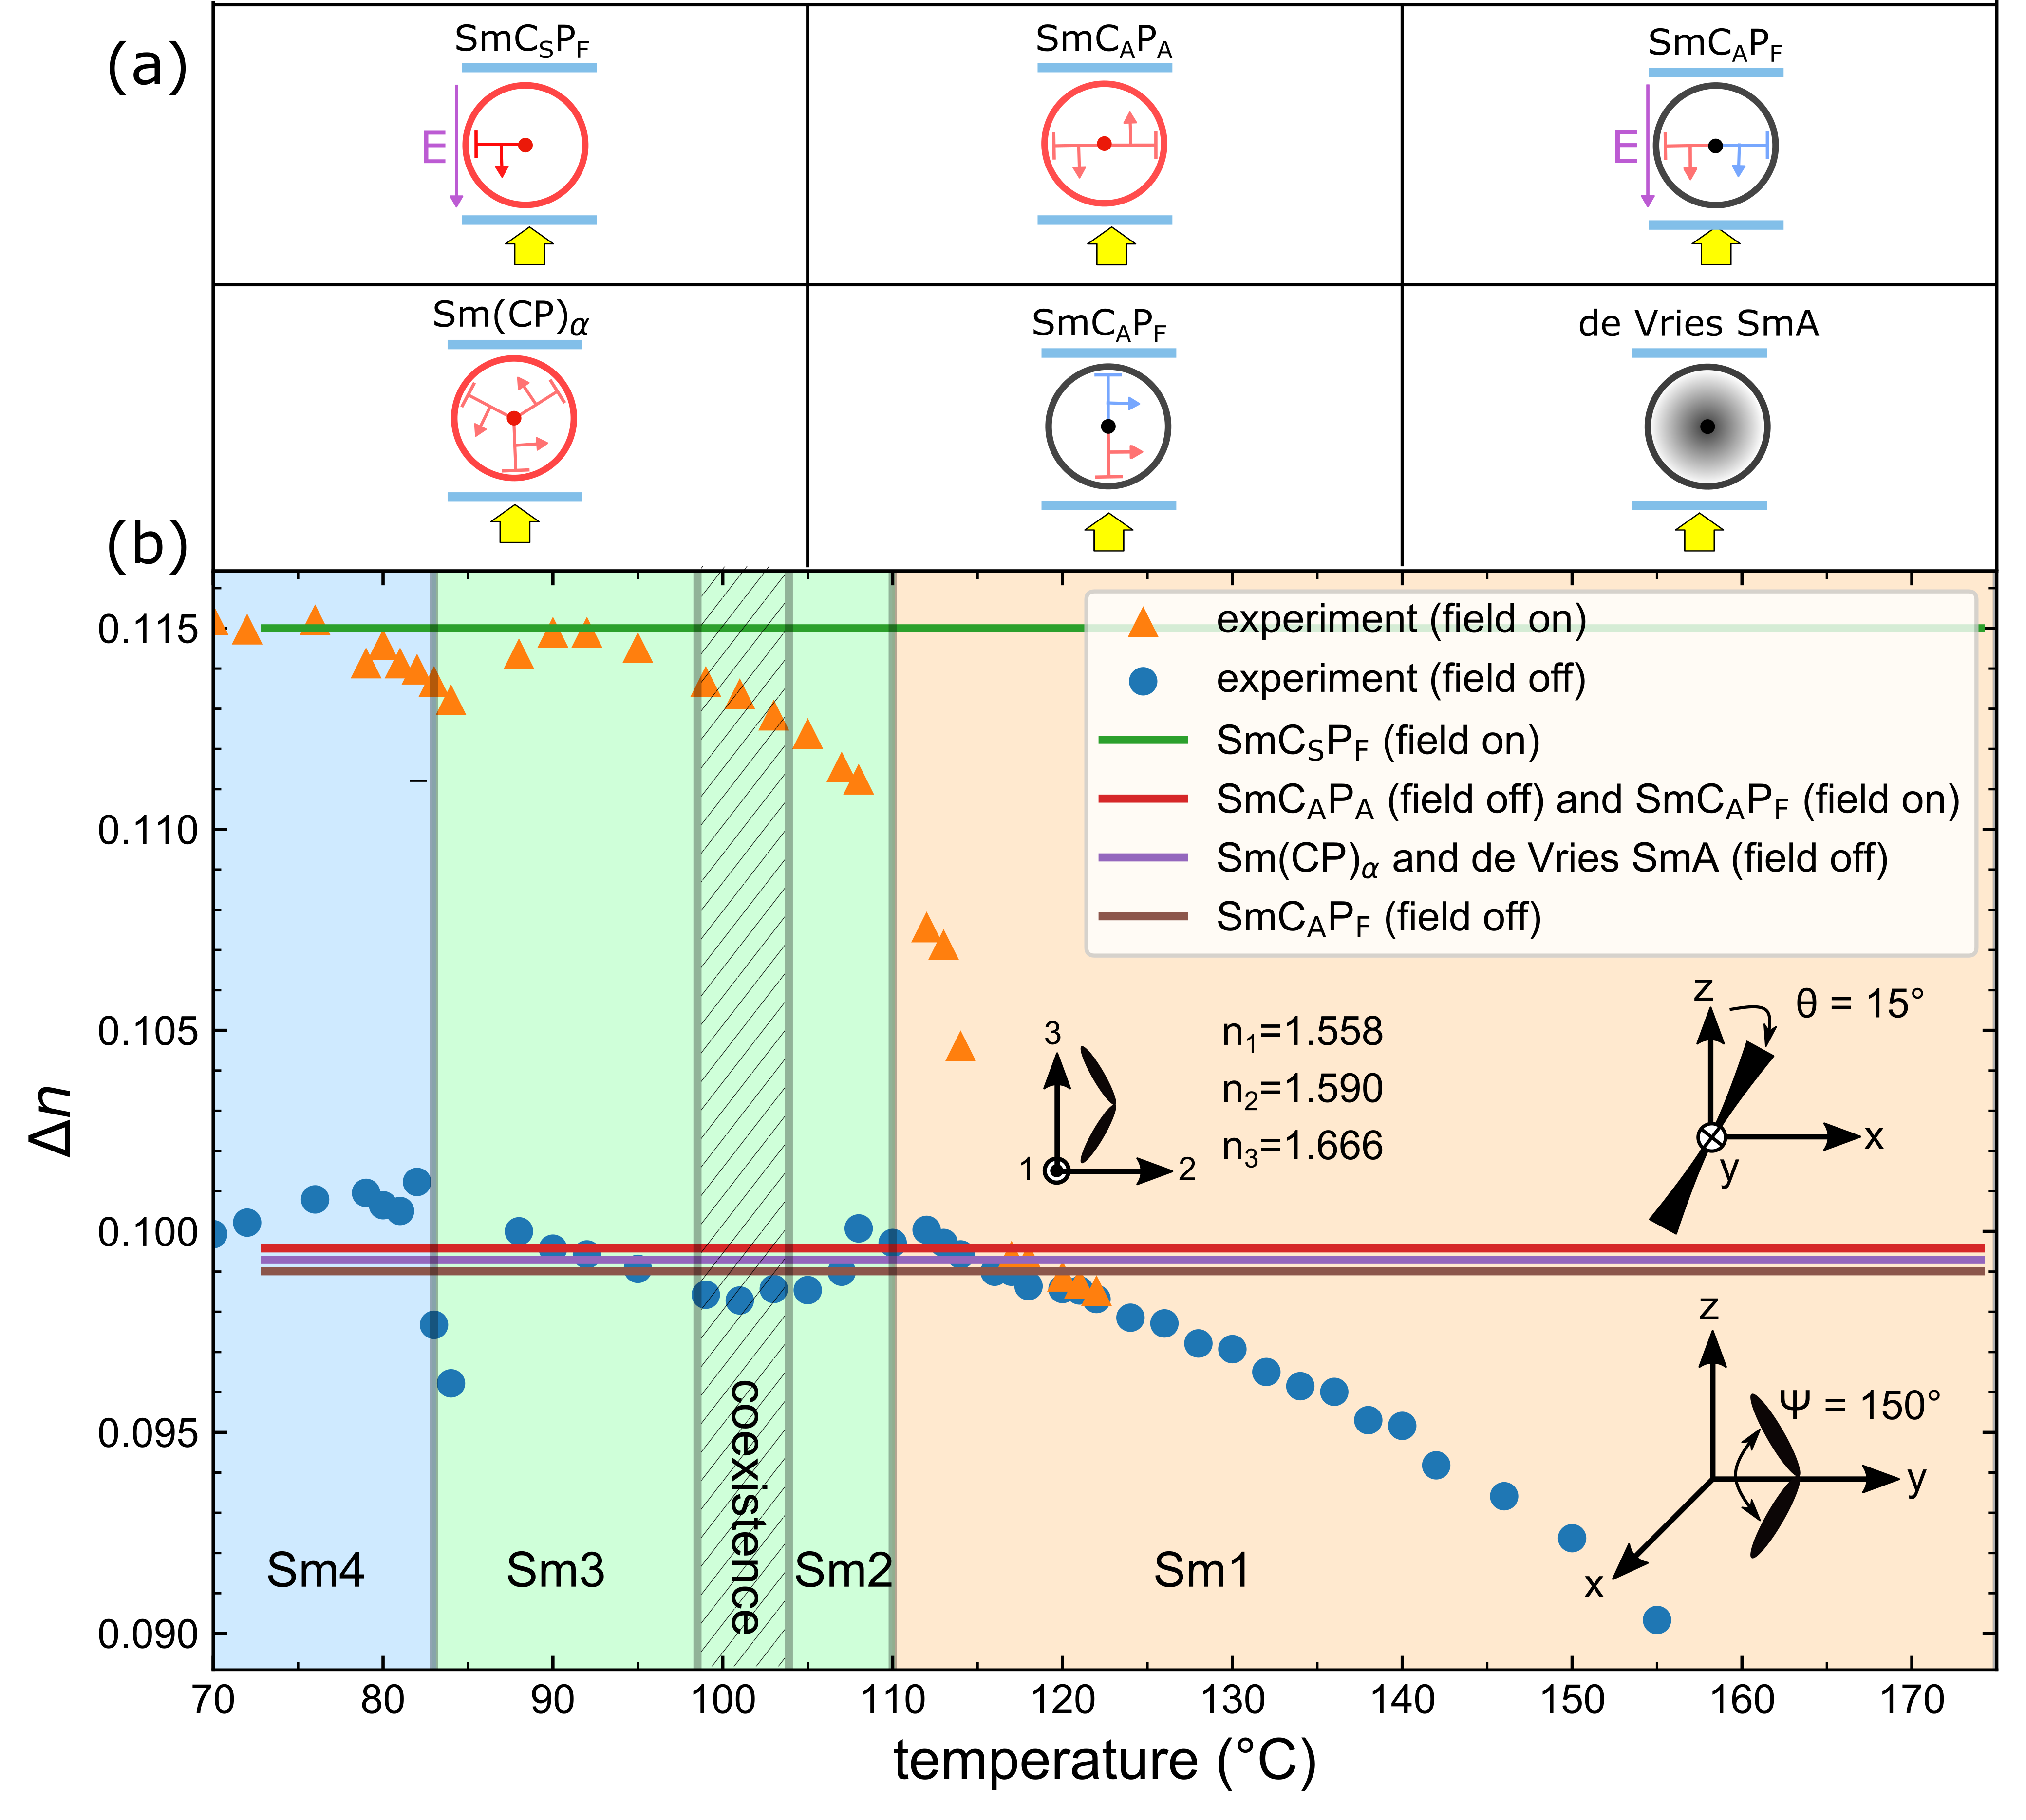
\includegraphics[width=1\linewidth]{theory-biref.png}
    \caption{\label{fig:calbif} The calculated birefringence for various model
        banana phases assuming
        an opening angle, $\Psi = \SI{150}{\degree}$ and molecular tilt, $\theta
        = \SI{15}{\degree}$ compared with the experimentally observed birefringence. (a) Schematic cross-sections of various smectic phases in a cell with bookshelf geometry. For
    chiral phases, the tilt-cone is red, while for achiral phases it is black.
    (b) Measured and calculated birefringence vs temperature. The birefringence
    is computed using indices of refraction chosen for the best fit to the
    experiment: $n_1=1.59$, $n_2=1.558$, $n_3=1.666$.
    The birefringence is computed using the method described by
Shen \textit{et al.}~\cite{shen2013generalized}.}
\end{figure}
%
\begin{figure}[H]
    \centering
    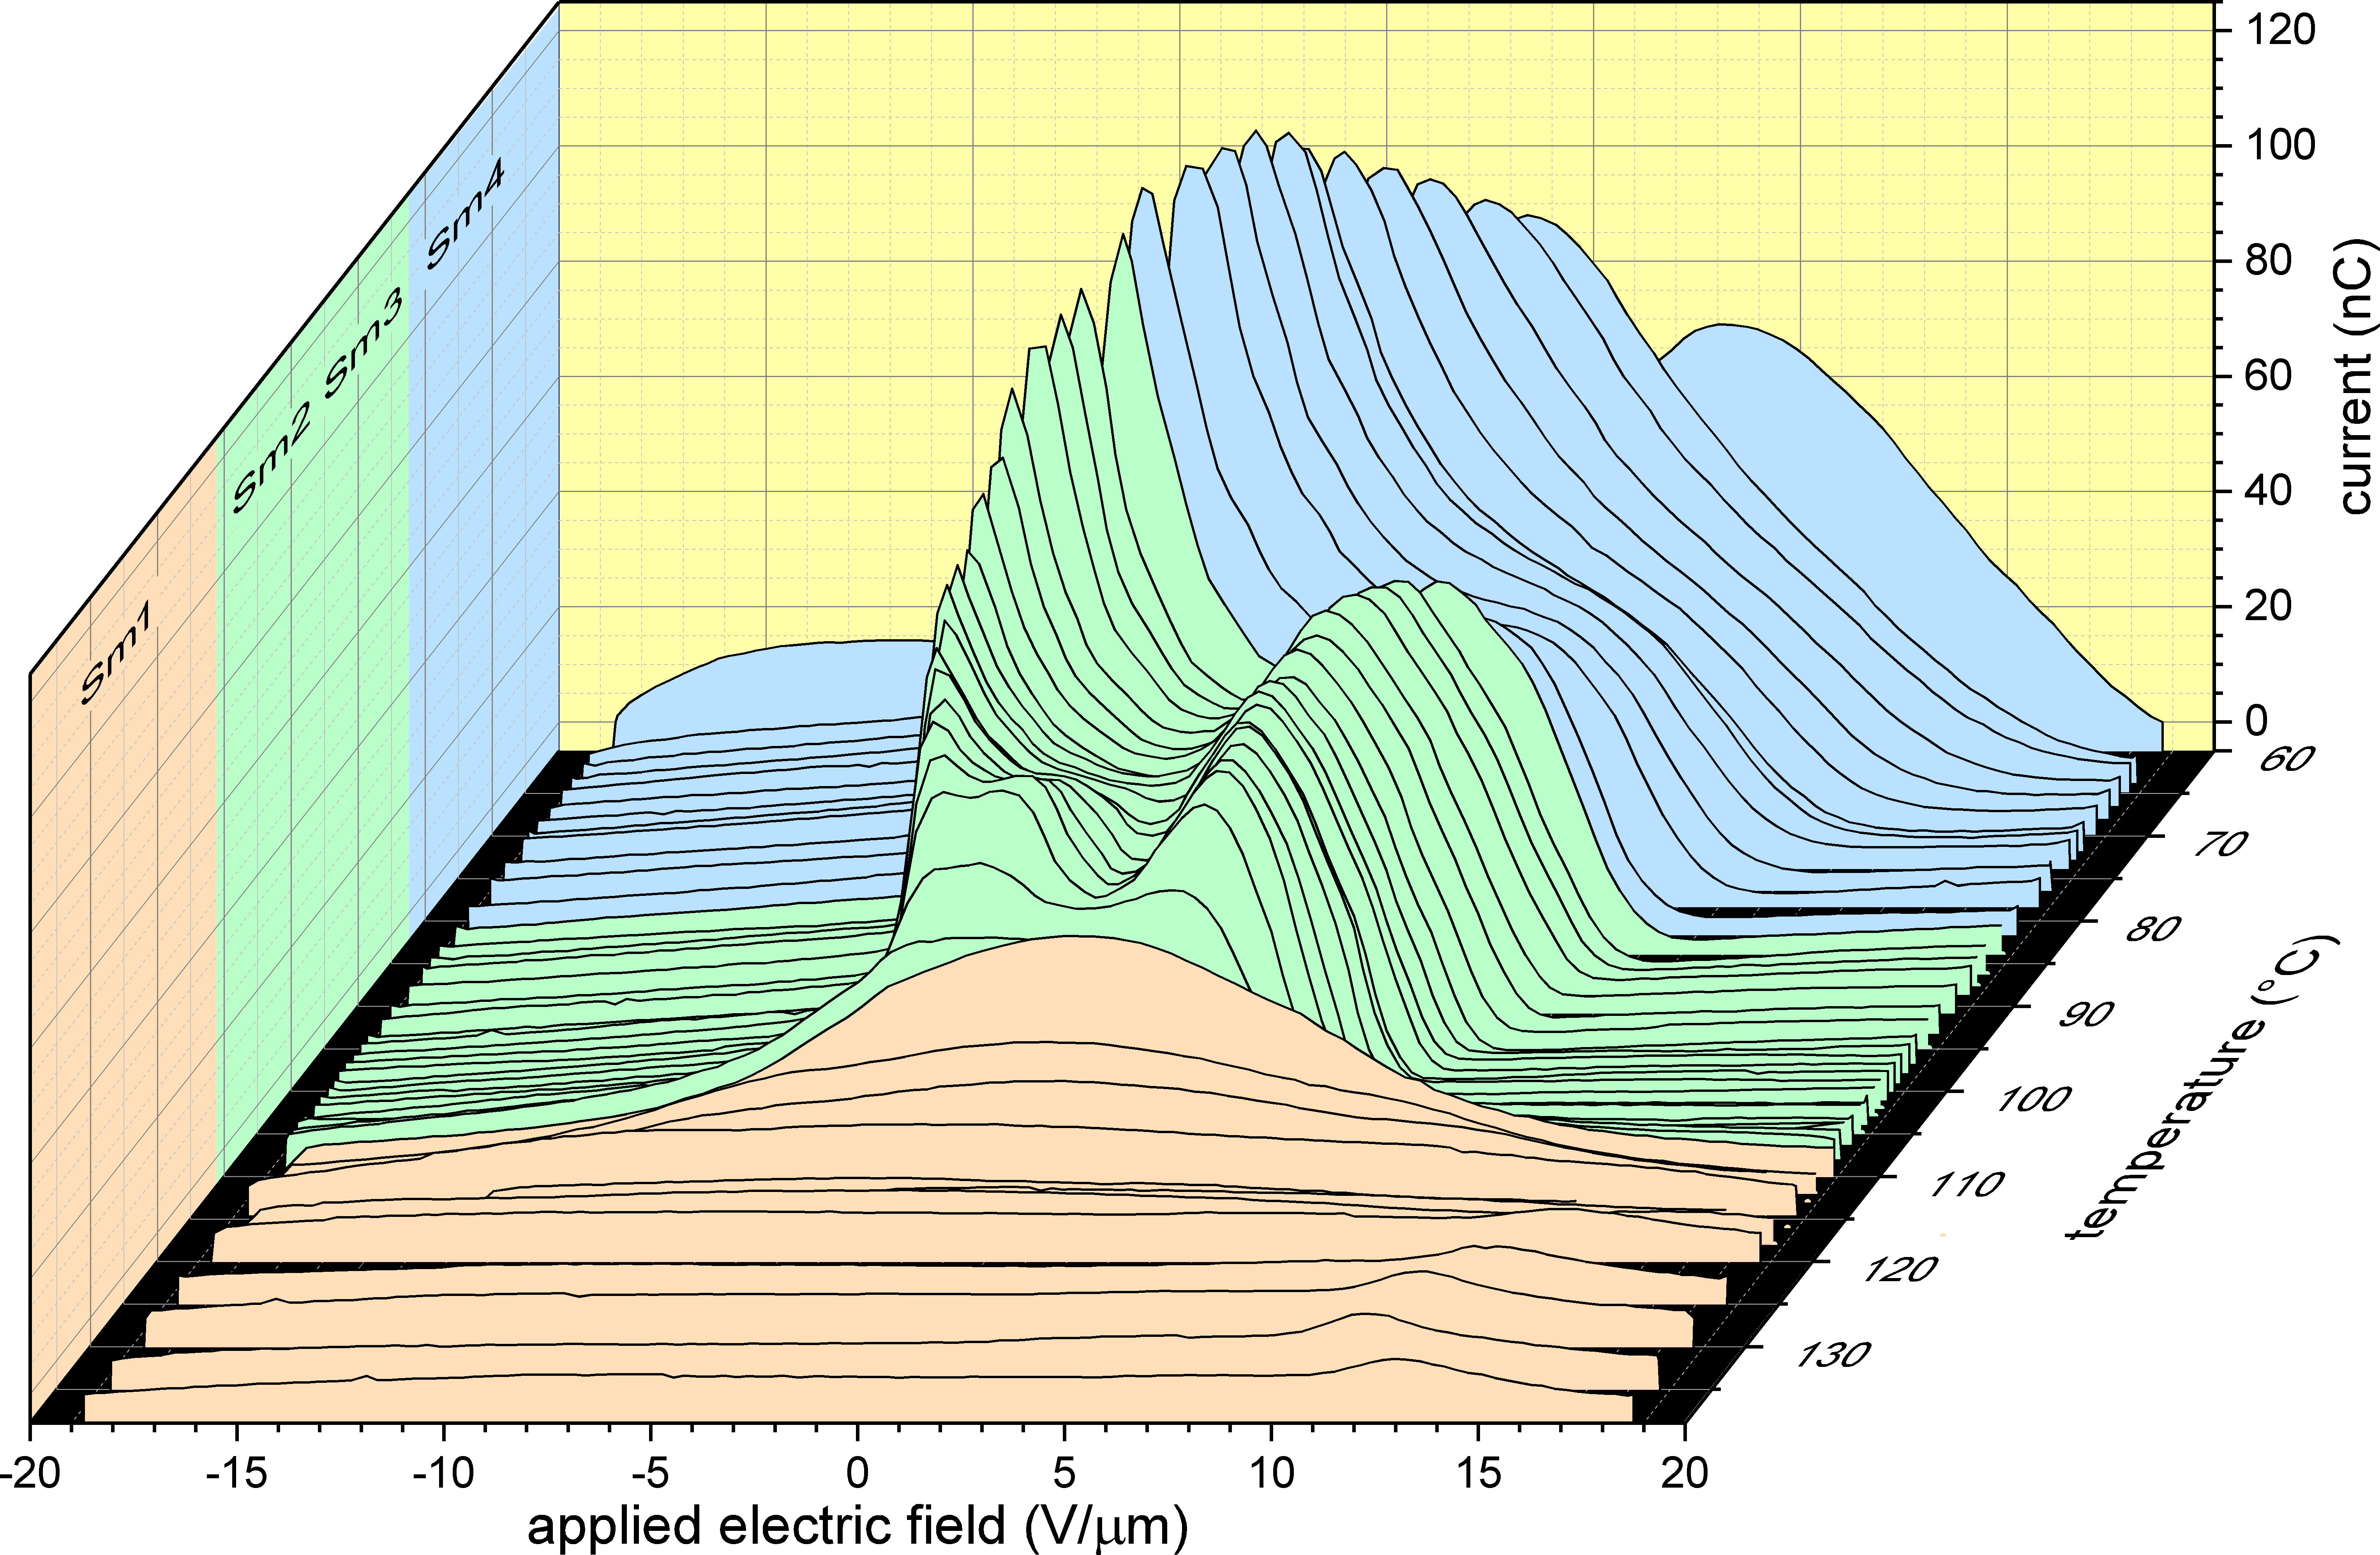
\includegraphics[width=.9\textwidth]{polzv9.png}

    \caption{Polarization current response of a \SI{4.5}{\micro\metre}-thick \nfour{phi} sample in an Instec cell subjected  to a \SI{40}{\hertz} triangular voltage with an amplitude of \SI{72}{\volt}.
The current response, $I = dP/dt$ in the Sm1 phase is a single, broad hump
corresponding to the field-induced alignment of the initially random polarization.
The Sm1 phase becomes a chiral \smcspf{phi} when the polarization orientation saturates
(when $I(V)$ goes to zero). As the temperature is lowered, this peak splits into
sub-peaks, indicating internal stabilization of a state or states of lower
polarization, which optical and RSoxS observation show to be the incommensurate
\smchph{phi} helix of  SmCP layers in the Sm2 phase and bilayer
\smcapa{phi} antiferroelectric ordering of SmCP layers in the Sm3 phase.
In the Sm2  phase, two current peaks appear during the rewinding of the helix as the
magnitude of the applied field falls to zero. The right current peak (as the
applied field increases again) marks the transition from the ground state of \smchph{phi} to the field-aligned \smcspf{phi}. Three polarization switching peaks are indicative of ferrielectricity (see the discussion of the SmC$^{*}_\textrm{FI1}$ calamitic phase in Takezoe et~al.~\cite{takezoe2010antiferroelectric}), and would be expected as the measured pitch of the Sm2 phase ($2.8$ layers) is close to the pitch of the quintessential ferrielectric phase, the SmC$^{*}_\textrm{FI1}$ ($3$ layers).
In the Sm3 phase, the left and right hand peaks mark the transitions from the \smcspf{phi}-up to \smcapa{phi}, and \smcapa{phi} to
\smcspf{phi}-down, respectively.
The transition to the Sm4 phase is marked by the appearance of a pattern of low birefringence (yellow) and high birefringence
(orange) domains and a single current peak that moves continuously to $V=0$,
with a broad current `shoulder' on the right. A current peak at $V = 0$ is characteristic of field-driven
uniform, ``block'' reorientation of a ferroelectric polarization distribution, indicating the
development of layer interactions that prefer \smcapf{phi} over \smcapa{phi},  the former being achiral as Figure~1(k--m) indicates. At zero field, the \smcapf{phi} polarization is parallel to the glass, giving the low-birefringence, yellow domains seen in Figure~1(l). The orange domains remain from the field application (Figure~1(k)), indicating that these regions stay in the \smcapf{phi}-up state until field reversal converts them into the \smcapf{phi}-down state, also orange (Figure~1(m)). The `shoulder' in this current peak results from the reorientation of these pinned domains. The liquid crystal phases are indicated schematically using the same color scheme as in Figure~1.\label{fig:polz}}
\end{figure}

\begin{figure}[H]
    \centering
    \includegraphics[width=.85\textwidth]{montageForSupp.pdf}
    \caption{Polarization current response vs.\ time of a \SI{4.5}{\micro\metre}-thick \nfour{phi} sample in an Instec cell subjected  to a \SI{40}{\hertz} triangular voltage with an amplitude of \SI{72}{\volt}. The data are the same as in Figure~\ref{fig:polz}.}
\end{figure}

\begin{figure}[H]
    \centering
    \includegraphics[width=.85\textwidth]{montagevVsCForSupp.pdf}
    \caption{Polarization current response vs.\ applied field of a \SI{4.5}{\micro\metre}-thick \nfour{phi} sample in an Instec cell subjected  to a \SI{40}{\hertz} triangular voltage with an amplitude of \SI{72}{\volt}. The data are the same as in Figure~\ref{fig:polz}.
    The blue and orange curves correspond respectively to the polarization current measured with an increasing and decreasing applied voltage.}
\end{figure}

\begin{figure}[H]
    \centering
    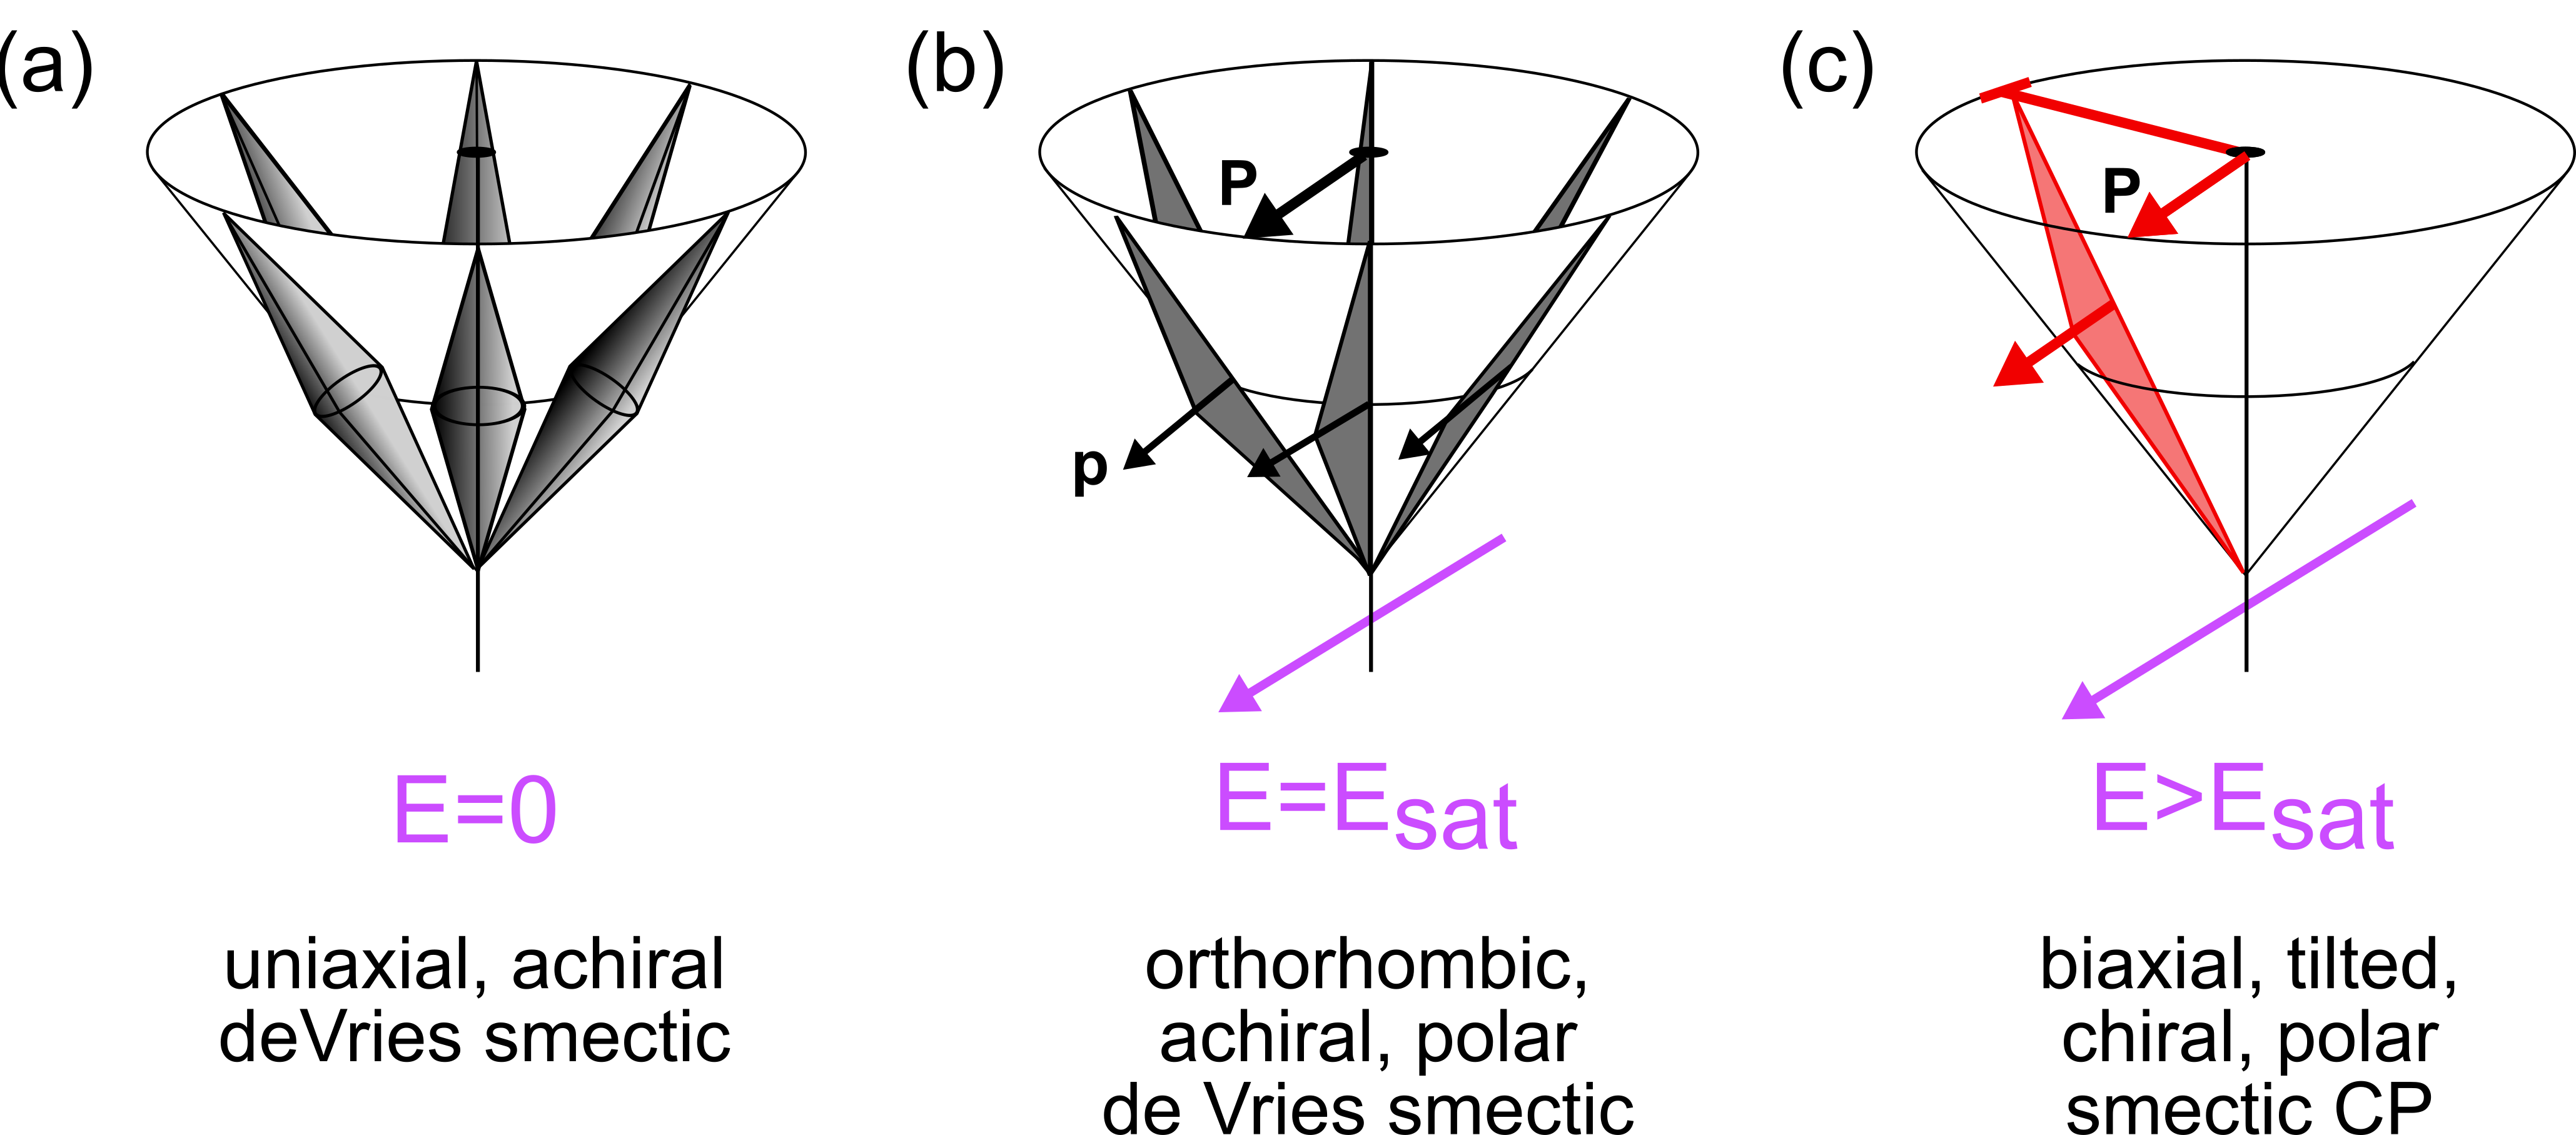
\includegraphics[width=.7\textwidth]{dvAlign.png}
    \caption{Response of the Sm1 phase to an applied electric field. (a) At zero
    field, the Sm1 is a uniaxial, achiral de Vries smectic, where the tilt and
    polar order are azimuthally distributed. (b) Application of an electric field
begins to align the polar director, though the tilt remains azimuthally
distributed, giving a polar but achiral bent-core structure. (c) When the
applied field is larger than the saturation value ($E_\text{sat}$), the tilt
also aligns, giving a biaxial, tilted, polar and chiral bent-core structure.}
\end{figure}

%\FloatBarrier
\bibliography{pal30.bib}
\end{document}
